\documentclass[tikz,border=8pt]{standalone}
% Shared look for every TikZ diagram. Load with % Shared look for every TikZ diagram. Load with % Shared look for every TikZ diagram. Load with \input{../../tools/tikz-style.tex}
\usepackage[T1]{fontenc}
\usepackage{lmodern}
\renewcommand{\sfdefault}{lmr}  % diagrams use the same serif as the text
\usetikzlibrary{arrows.meta, positioning, shapes.geometric, calc, fit, backgrounds}
\definecolor{cblue}{HTML}{4C78A8}
\definecolor{corange}{HTML}{F58518}
\definecolor{cgreen}{HTML}{54A24B}
\definecolor{cred}{HTML}{E45756}
\definecolor{cpurple}{HTML}{B279A2}
\definecolor{cgrey}{HTML}{6B6B6B}
\tikzset{
  every picture/.style={font=\sffamily, line width=1.2pt},
  box/.style={draw=#1, fill=#1!12, rounded corners=4pt, align=center, inner sep=7pt, minimum height=1.1cm},
  box/.default=cgrey,
  arrow/.style={-{Stealth[length=3mm]}, draw=cgrey, line width=1.4pt},
  title/.style={font=\sffamily\bfseries\Large},
  note/.style={font=\sffamily\small, text=cgrey, align=center},
}
\AtBeginDocument{\hyphenpenalty=10000 \exhyphenpenalty=10000}

\usepackage[T1]{fontenc}
\usepackage{lmodern}
\renewcommand{\sfdefault}{lmr}  % diagrams use the same serif as the text
\usetikzlibrary{arrows.meta, positioning, shapes.geometric, calc, fit, backgrounds}
\definecolor{cblue}{HTML}{4C78A8}
\definecolor{corange}{HTML}{F58518}
\definecolor{cgreen}{HTML}{54A24B}
\definecolor{cred}{HTML}{E45756}
\definecolor{cpurple}{HTML}{B279A2}
\definecolor{cgrey}{HTML}{6B6B6B}
\tikzset{
  every picture/.style={font=\sffamily, line width=1.2pt},
  box/.style={draw=#1, fill=#1!12, rounded corners=4pt, align=center, inner sep=7pt, minimum height=1.1cm},
  box/.default=cgrey,
  arrow/.style={-{Stealth[length=3mm]}, draw=cgrey, line width=1.4pt},
  title/.style={font=\sffamily\bfseries\Large},
  note/.style={font=\sffamily\small, text=cgrey, align=center},
}
\AtBeginDocument{\hyphenpenalty=10000 \exhyphenpenalty=10000}

\usepackage[T1]{fontenc}
\usepackage{lmodern}
\renewcommand{\sfdefault}{lmr}  % diagrams use the same serif as the text
\usetikzlibrary{arrows.meta, positioning, shapes.geometric, calc, fit, backgrounds}
\definecolor{cblue}{HTML}{4C78A8}
\definecolor{corange}{HTML}{F58518}
\definecolor{cgreen}{HTML}{54A24B}
\definecolor{cred}{HTML}{E45756}
\definecolor{cpurple}{HTML}{B279A2}
\definecolor{cgrey}{HTML}{6B6B6B}
\tikzset{
  every picture/.style={font=\sffamily, line width=1.2pt},
  box/.style={draw=#1, fill=#1!12, rounded corners=4pt, align=center, inner sep=7pt, minimum height=1.1cm},
  box/.default=cgrey,
  arrow/.style={-{Stealth[length=3mm]}, draw=cgrey, line width=1.4pt},
  title/.style={font=\sffamily\bfseries\Large},
  note/.style={font=\sffamily\small, text=cgrey, align=center},
}
\AtBeginDocument{\hyphenpenalty=10000 \exhyphenpenalty=10000}

% Multivariate chain rule: t affects f along two paths, through x1 and through x2. Multiply along each path, add the paths.
\begin{document}
\begin{tikzpicture}[node distance=1.2cm and 4.2cm, every node/.append style={font=\large}]
  \node[box=cgrey, minimum width=1.4cm] (t) {$t$};
  \node[box=cblue, minimum width=2.6cm, above right=0.5cm and 3.6cm of t] (x1) {$x_1 = \cos t$};
  \node[box=cblue, minimum width=2.6cm, below right=0.5cm and 3.6cm of t] (x2) {$x_2 = \sin t$};
  \node[box=corange, minimum width=1.4cm, below right=0.5cm and 3.6cm of x1] (f) {$f(x_1, x_2)$};
  \draw[arrow] (t) -- node[above left, font=\large] {$\dfrac{dx_1}{dt}$} (x1);
  \draw[arrow] (t) -- node[below left, font=\large] {$\dfrac{dx_2}{dt}$} (x2);
  \draw[arrow] (x1) -- node[above right, font=\large] {$\dfrac{\partial f}{\partial x_1}$} (f);
  \draw[arrow] (x2) -- node[below right, font=\large] {$\dfrac{\partial f}{\partial x_2}$} (f);
  \node[below=0.9cm of x2, font=\large] {$\dfrac{df}{dt} = \underbrace{\dfrac{\partial f}{\partial x_1}\dfrac{dx_1}{dt}}_{\text{path through } x_1} + \underbrace{\dfrac{\partial f}{\partial x_2}\dfrac{dx_2}{dt}}_{\text{path through } x_2}$};
\end{tikzpicture}
\end{document}
